\documentclass{standalone}
\usepackage{tikz}       % load in the tikz package for drawing figures

\begin{document}

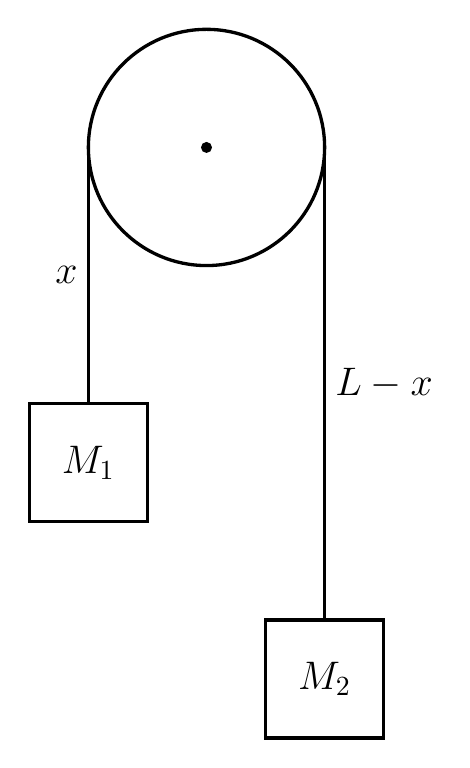
\begin{tikzpicture}[very thick, font=\Large]     % start of the drawing

    \draw (0, 0) circle[radius=1.5];
    \fill (0, 0) circle[radius=0.07];

    % draw the rope to the first and second weight
    \draw (-1.5, 0) -- (-1.5, -3.25) node[pos=0.5, left] {$x$};
    \draw (1.5, 0) -- (1.5, -6.0) node[pos=0.5, right] {$L-x$};

    % draw the weights as rectangles
    \node[draw, rectangle, anchor=center, minimum size=1.5cm] at (-1.5, -4.0) {$M_1$};
    \node[draw, rectangle, anchor=center, minimum size=1.5cm] at (1.5, -6.75) {$M_2$};
\end{tikzpicture}

\end{document}
